\documentclass[a4paper,14pt]{extarticle}
\usepackage[english,russian]{babel}
\usepackage[cache=false]{minted}
\usepackage{fontspec}
\usepackage{indentfirst}
\usepackage{listings}
\usepackage{color}
\usepackage{caption}
\usepackage{amsmath}
\usepackage{hyperref}
\usepackage{graphicx}
\usepackage[%
    left=20mm,%
    right=10mm,%
    top=20mm,%
    bottom=20mm,%
]{geometry}%
\usepackage{titlesec}


\setmainfont{PT Astra Serif}

\hypersetup{
    colorlinks=true,
    linkcolor=black,
    filecolor=magenta,
    urlcolor=cyan,
    pdftitle={Лабораторная работа №4},
    pdfpagemode=FullScreen,
}

\newcommand{\hlink}[2]{\href{#1}{\color{blue}\underline{#2}}}
\graphicspath{ {./images/} }

\setmonofont[Scale=0.8]{JetBrains Mono}
\setminted{frame=lines, framesep=3mm, fontsize=\small}
\usemintedstyle{vs}

\titleformat{\section}
{\normalfont\bfseries}{}{0pt}{Упражнение \thesection.\;}

\numberwithin{figure}{section}

\begin{document}

\begin{titlepage}
    \vspace{0pt plus2fill}
    \noindent

    \vspace{0pt plus6fill}
    \begin{center}
        \textbf{\large{Санкт-Петербургский национальный исследовательский университет информационных
                технологий, механики и оптики}}

        \vspace{0pt plus2fill}
        \textbf{\Large{ЛАБОРАТОРНАЯ РАБОТА №2}}

        \vspace{0pt plus2fill}
        \textbf{\large{Создание и использование структуры}}
    \end{center}

    \vspace{0pt plus8fill}
    \begin{flushright}
        Студент: \\
        \textit{Швалов Даниил Андреевич}

        \textit{Факультет ИКТ}

        Группа: \textit{К32211}

        Преподаватель: \\
        \textit{Иванов Сергей Евгеньевич}
    \end{flushright}

    \vspace{0pt plus4fill}
    \begin{center}
        {Санкт-Петербург~--- 2023}
    \end{center}
\end{titlepage}

\section{Создание перечисления}

Проделав все шаги, перечисленные в задании, получим следующий исходный код:

\inputminted{csharp}{../BankAccount/BankAccount/Program.cs}

Результат работы программы представлен на рис. \ref{fig:task-1}.

\begin{figure}[H]
    \centering
    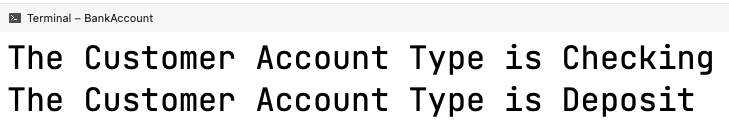
\includegraphics[width=0.7\textwidth]{images/task-1.png}
    \caption{Вывод программы BankAccount}
    \label{fig:task-1}
\end{figure}

\section{Создание и использование структуры}

Выполнив все шаги из задания, получился следующий исходный код:

\inputminted{csharp}{../StructType/StructType/Struct.cs}

Запустив его, получим вывод, изображенный на рис. \ref{fig:task-2-1}.

\begin{figure}[H]
    \centering
    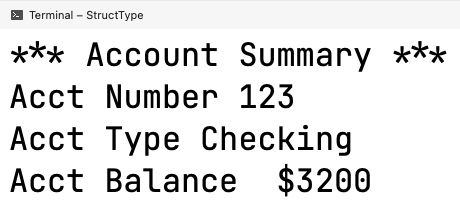
\includegraphics[width=0.7\textwidth]{images/task-2-1.png}
    \caption{Вывод программы Struct}
    \label{fig:task-2-1}
\end{figure}

Доработав программу и добавив ввод пользовательских данных, получим следующую программу:

\inputminted{csharp}{../StructType/StructType/Struct1.cs}

Запустив доработанную программу, получим результат, показанный на рис. \ref{fig:task-2-2}.

\begin{figure}[H]
    \centering
    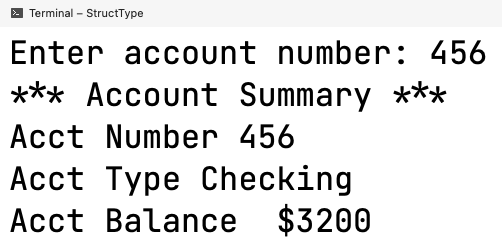
\includegraphics[width=0.7\textwidth]{images/task-2-2.png}
    \caption{Вывод программы доработанной Struct}
    \label{fig:task-2-2}
\end{figure}

\section{Реализация структуры Distance}

Согласно заданию считываем значения длин в дюймах с стандартного ввода. После этого записываем значение дюймов в каждое из двух расстояний, а в третье расстояние записываем их сумму также в дюймах. Затем для каждой структуры пересчитываем дюймы в футы. В конце концов, выводим значение расстояний на экран в заданном формате (см. рис. \ref{fig:task-3}).

\inputminted{csharp}{../Distance/Distance/Program.cs}

\begin{figure}[H]
    \centering
    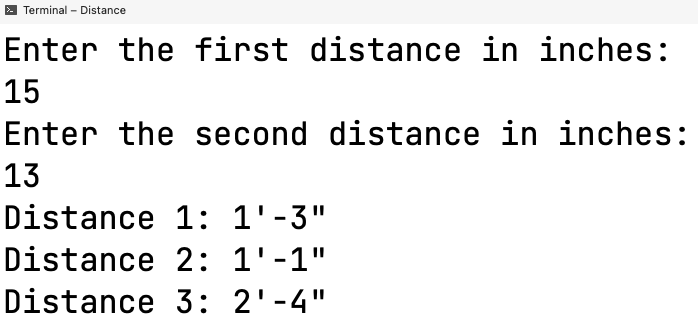
\includegraphics[width=0.7\textwidth]{images/task-3.png}
    \caption{Вывод программы Distance}
    \label{fig:task-3}
\end{figure}

\end{document}
